\chapter{Конструкторский раздел}
В этом разделе приводится подробное описание разрабатываемого метода,
выделяются основные его компоненты, описываются метрики, оценивающий метод. Так же приводится описание ПО, собирющее данные для анализа.
\subsection{Метод обнаружения аномалий}
В выводе аналитической части предлагается разработать новый метод обнаружения аномалий. Новый метод будет является результатом ансамблирования трех метрических методов.
На вход методу подается файл с нормализованными значениями атрибутов, с фиксированным заранее известным количеством атрибутов для каждого элемента. Временная отметка элемента представляется в качестве отдельного нормализованного атрибута.
\subsection{Локальный коэффииент выбросов}
Этот метод описан в аналитической части. В результате его работы для каждого элемента набора устанавливается метка, позволяющая однозначно классифицировать принадлежность элемента к аномальным.

\subsection{Компонентный коэффициент выбросов}
Для подсчета метрики COF используется следующая формула:
\begin{equation}
L=\sum_{0}^{k}x_j0 - x_ji
\end{equation}
\subsection{Ансамблирование методов}
Каждый из вышеописанных методов инвариантен и иммутабелен относительно набора данных. В результате их работы получается три набора меток. На основе этих наборов формируется финвальный набор меток по следующему принципу: если элемент имеет две или более "аномальных" метки, то ему присвается "аномальная" метка, иначе - "нормальная" метка.
\subsection{Анализ резульатов работы методов}
Для проверки рабоспобности метода его нужно оценить при помощи наборов данных. Метрикой сравнения наборов данных был выбран AUC ROC — площадь под графиком, позволяющим оценить качество бинарной классификации, отображающим соотношение между долей объектов от общего количества носителей признака, верно классифицированных как несущих признак, и долей объектов от общего количества объектов, не несущих признака, ошибочно классифицированных как несущих признак. 
\begin{figure}
	\centering
	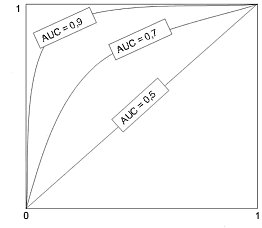
\includegraphics[width=.5\textwidth]{img/aucROc.png}
	\caption{Auc ROC}\label{cha:design}
	\label{fig06}
\end{figure}
При помощи этой метрики планируется оценить адекватность работы алгоритма на размеченных наборах данных и  сравнить  с другими методами.
\subsection{Собирающее данные для анализа ПО}
Для применения метода на практике было разработано ПО, которое позволяет собирать данные для анализа(телеметрию). В состав приложения будет входить плагин для графического редактора, backend-сервер, frontend. Так же на бекенде будет размещена база данных где будут размещаться "сырые" данные. 
\begin{figure}
	\centering
	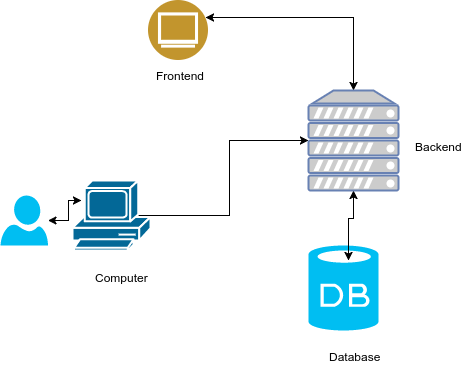
\includegraphics[width=.5\textwidth]{img/diagram1.png}
	\caption{Общая архитектура приложения}\label{cha:design}
	\label{fig07}
\end{figure}
Результатом работы ПО будет неразмеченный набор данных, содержащий фиксированное количество атрибутов.
\subsubsection{Собираемые данные}
Основые собираемые данные приведены в таблице \ref{tab:collectdata}:

\begin{table}[!h]

\caption{\label{tab:collectdata}Описание собираемых данных}

\begin{center}

\begin{tabular}{|l|l|l|}

\hline

Информация о & Источник данных & Данные \\

\hline \hline

Инструменты & KisTool::activate, KisTool:deactivate & 

CountUse float64 

\tabularnewline & & Time     float64 

\tabularnewline & & ToolName string 

\tabularnewline & & Timestamp     float64 \\


\hline

Действия & 

KisMainWindows actioncollection()

& 

CountUse float64 

\tabularnewline & & TimeUse      float64 

\tabularnewline & & ActionName string \\


\hline

Cвойства изображений & 

KisDocument::saveFile()

& 

ColorProfile string 

\tabularnewline & &  ColorSpace   string 

\tabularnewline & & Height       float64 

\tabularnewline & & Width      float64

\tabularnewline & & Size      float64 

\tabularnewline & & NumLayers      float64 

\tabularnewline & & Timestamp     float64 \\


\hline

Информация  &

KisDocument::saveFile()	& 

AppVersion string 

\tabularnewline о компьютере & &  CompilerVersion   string 

\tabularnewline & & CompilerType      string 

\tabularnewline & & CpuArchitecture      string

\tabularnewline & & CpuCount     float64 

\tabularnewline & & CpuFamily      float64  

\tabularnewline & & CpuIsIntel    bool 

\tabularnewline & & CpuModel      float64  

\tabularnewline & & LocaleLanguage      string

\tabularnewline & & OpenGlGlslVersion     string

\tabularnewline & & OpenGlRenderer     string   

\tabularnewline & & OpenGlVendor    string 

\tabularnewline & & PlatformOs    string 

\tabularnewline & & PlatformVersion    string 

\tabularnewline & & QtVersion    string    

\tabularnewline & & ScreenDpi    string 

\tabularnewline & & ScreenHeight    string

\tabularnewline & & ScrennWidth    string 

\tabularnewline & & Timestamp     float64     \\            

\hline

Ассерты &

kis\_assert\_common()	& 

AssertFile string

\tabularnewline & &  AssertLine float64

\tabularnewline & & 	AssertText string

\tabularnewline & & 	Count float64

\tabularnewline & & 	IsFatal bool

\tabularnewline & & Timestamp     float64 \\

\hline

\end{tabular}

\end{center}

\end{table}
\subsubsection{Клиентская часть}
Был разработан плагин для графического редактора Krita, который позво­
ляет собирать телеметрию с пользователей. Телеметрия отправляется через опре­
деленные интервалы времени на удаленный сервер. Записи о действиях и инстру­
ментах отправляются каждые n минут. Информация о компьютере отправляется 1
раз при установке Krita. После этого в файл настроек записывается информация
о том, что больше информацию о компьютере отправлять не стоит. Это позволяет
избежать "замусоривания"отправляемой информации за счёт отсуствия дублирова­
ния. Информация об ассертах отправляется по мере необходимости. Если программа
находится debug-режиме, программа аварийно завершает свою работу после любого
ассерта. После того как аварийный ассерт сработал, он записывается в файл конфига Krita. При следующей запуске программы, он будет прочитан оттуда и отправлен на удаленный сервер при старте программы. Если программа собрана в release-версии, то при ассерте, не приводящем к аварийному завершению программы, информация об ассерте в рантайме программы отправляется на удаленный сервер. Собираемые метрики агрегруются на стороне клиента в http-запрос. Пример тела запроса представляет собою JSON, пример этого JSON приведен ниже(форматирование нарушено в целях наглядности).
\begin{lstlisting}[language=c++,,escapeinside={(@}{@)},caption={Тело http-запроса}] 
{
"Name": [
{
"Param1": 1,
"Param2": 4581,
"Timestamp": 12214
},
\end{lstlisting}
\subsubsection{Серверная часть}
На сервере метрики обработываются и заносятся в JSON виде "как есть". 
Сервер умеет отдавать метрики в нормализованном виде за опредленный промежуток времени, а так же
\subsubsection{Динамическое изменение данных}
Инструменты и действия(actions) могут меняться достаточно часто в про­
цессе разработки графическего редактора. Поэтому неразумно задавать статически
эти метрики в коде. В коде бекенд-сервера реализована поддержка добавления но­
вых элементов. Раз в сутки просыпается новая горутина(легковесный тред), которая пробегается по базе данных и ищет новые инструменты и действия. После этого она записывает их в текстовый файл. Подобное разумно применять не только для инструментов и действий, но и для любых часто изменяющихся данных.  В будущем возможно расширения этой системы.